% ACTIVIDAD 1 — MAPA CONCEPTUAL
% Investigación aplicada a la contaduría / UAS
\documentclass[spanish,letterpaper,oneside]{article}

\def\documenttitle {Reglas y estrategias para la escritura de textos académicos}
\def\documentsubtitle {Mapa conceptual a partir de la comprensión lectora}
\def\documentsubject {Actividad 1 — Tema I}
\def\documentauthor {Martín Jonathan De La Cruz Muñoz}
\def\coursename {Investigación aplicada a la contaduría}
\def\coursecode {Grupo 101}
\def\universityname {Universidad Autónoma de Sinaloa}
\def\universityfaculty {Licenciatura en Contaduría Pública — Modalidad Virtual}
\def\universitydepartment {Facultad de Contaduría y Administración Culiacán}
\def\universitydepartmentimage {UAS/licenciatura-en-contaduria-uas/fcauas-logo.jpg}
\def\universitydepartmentimagecfg {height=1.45cm}
\def\universitylocation {Culiacán, Sinaloa, México}
\def\authortable {
  \begin{tabular}{ll}
    \textbf{Estudiante:} & Martín Jonathan De La Cruz Muñoz \\
    Matrícula: & 26031061 \\
    \textit{Docente:} & Dra. Nadia Aileen Valdez Acosta \\
    Grupo: & 101 \\
    Plan y ciclo: & Plan 22 — Ciclo 2026 \\
    Fecha de realización: & \today \\
    Lugar: & \universitylocation
  \end{tabular}
}

\input{template}
\usepackage{helvet}
\renewcommand{\familydefault}{\sfdefault}
\usepackage{tikz}
\usetikzlibrary{arrows.meta,calc,fit,positioning,shadows.blur,shapes.geometric}
\setcitestyle{authoryear,open={(},close={)}}

\definecolor{uasBlueDark}{HTML}{0B294C}
\definecolor{uasBlue}{HTML}{123B6D}
\definecolor{uasBlueLight}{HTML}{E9F0F8}
\definecolor{uasGold}{HTML}{C79A2B}
\definecolor{uasGreen}{HTML}{39725B}
\definecolor{uasGray}{HTML}{44546A}

\begin{document}
\templatePortrait
\templatePagecfg
\onehalfspacing

\begin{abstractd}
Este reporte organiza mediante un mapa conceptual las reglas y estrategias que permiten transformar la comprensión lectora en escritura académica. La propuesta relaciona lectura estratégica, planificación, textualización, revisión y documentación de fuentes como partes de un proceso recursivo. El criterio central es que un texto académico sólido no surge de copiar información, sino de seleccionar, jerarquizar, relacionar y reformular ideas con un propósito, una estructura coherente y atribución verificable.
\end{abstractd}

\templateIndex
\templateFinalcfg

\section{Introducción}

La escritura académica comienza antes de redactar la primera oración. Leer con un propósito, reconocer la tesis de una fuente, distinguir ideas principales de ejemplos y relacionar la información con conocimientos previos son operaciones que permiten decidir qué se escribirá y con qué fundamento. Por ello, comprensión y escritura no constituyen tareas aisladas: la lectura produce una representación del contenido y la escritura reorganiza esa comprensión para comunicar una idea propia.

Redactar tampoco es una secuencia rígida. El escritor planifica, produce texto y revisa, pero puede regresar a cualquiera de estas operaciones cuando descubre una relación nueva, una inconsistencia o una fuente insuficiente \citep{flowerHayesCognitiveProcess1981}. En el ámbito universitario, este proceso incluye reconocer la contribución de otras personas mediante citas y referencias. La atribución permite al lector diferenciar la voz propia de las ideas recuperadas y localizar las obras utilizadas \citep{apaCitasTexto2024,apaReferencias2023}.

El objetivo de esta actividad es representar las relaciones esenciales del Tema I mediante un mapa conceptual que responda la pregunta focal: \textit{¿cómo transforma la comprensión lectora la información de las fuentes en un texto académico claro, coherente y ético?}

\section{Criterio de construcción del mapa}

Un mapa conceptual representa conocimiento mediante conceptos jerarquizados y proposiciones formadas por conceptos unidos con palabras de enlace. Su calidad depende de que las conexiones expresen relaciones significativas, no únicamente proximidad gráfica \citep{novakCanasMapas2008}. A partir de este criterio se seleccionaron cinco núcleos: comprensión lectora, planificación, textualización, revisión y citación. Las conexiones cruzadas muestran que citar exige comprender la fuente, que revisar puede obligar a releer y que la coherencia depende tanto de planificar como de reformular.

\clearpage
\thispagestyle{empty}
\begin{landscape}
\begin{center}
{\Large\bfseries\color{uasBlueDark} Mapa conceptual del Tema I}\\[1mm]
{\small Pregunta focal: ¿cómo transforma la comprensión lectora la información de las fuentes en un texto académico claro, coherente y ético?}
\end{center}

\vspace{1mm}
\begin{center}
\begin{adjustbox}{max totalsize={0.99\linewidth}{0.75\textheight},center}
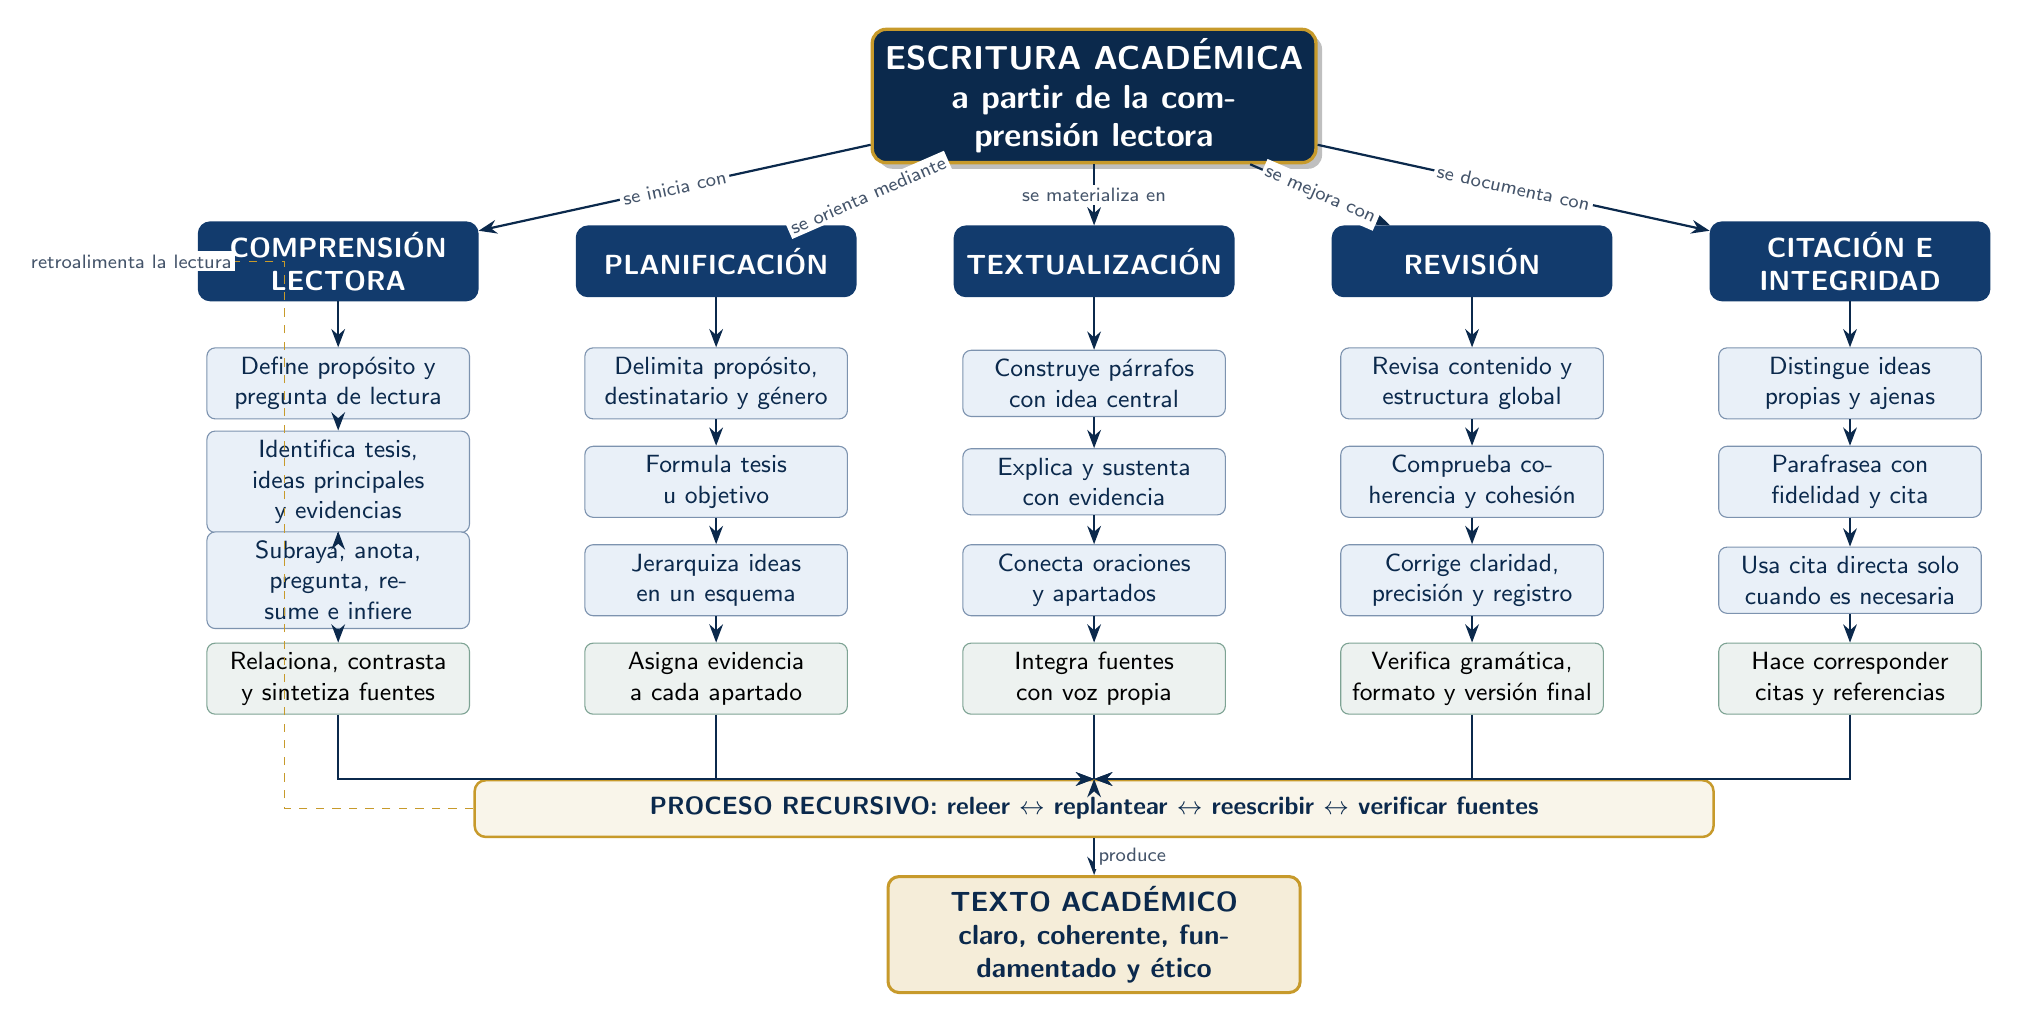
\begin{tikzpicture}[
  >=Stealth,
  root/.style={rounded corners=5pt,draw=uasGold,line width=1.2pt,fill=uasBlueDark,text=white,text width=5.4cm,minimum height=1.15cm,align=center,font=\bfseries\large,drop shadow},
  branch/.style={rounded corners=4pt,draw=uasBlue,line width=.9pt,fill=uasBlue,text=white,text width=3.30cm,minimum height=.88cm,align=center,font=\bfseries},
  concept/.style={rounded corners=3pt,draw=uasBlue!55,fill=uasBlueLight,text=uasBlueDark,text width=3.10cm,minimum height=.72cm,align=center,font=\small},
  evidence/.style={rounded corners=3pt,draw=uasGreen!65,fill=uasGreen!9,text=black,text width=3.10cm,minimum height=.72cm,align=center,font=\small},
  processbar/.style={rounded corners=4pt,draw=uasGold,line width=.9pt,fill=uasGold!10,text=uasBlueDark,text width=15.5cm,minimum height=.72cm,align=center,font=\small\bfseries},
  result/.style={rounded corners=4pt,draw=uasGold,line width=1.1pt,fill=uasGold!18,text=uasBlueDark,text width=5.0cm,minimum height=.90cm,align=center,font=\bfseries},
  link/.style={->,thick,draw=uasBlueDark},
  feedback/.style={->,semithick,dashed,draw=uasGold},
  label/.style={fill=white,inner sep=1.2pt,font=\scriptsize,text=uasGray,align=center}
]
\node[root] (root) at (0,0) {ESCRITURA ACADÉMICA\\a partir de la comprensión lectora};

\node[branch] (read) at (-9.6,-2.10) {COMPRENSIÓN\\LECTORA};
\node[branch] (plan) at (-4.8,-2.10) {PLANIFICACIÓN};
\node[branch] (write) at (0,-2.10) {TEXTUALIZACIÓN};
\node[branch] (review) at (4.8,-2.10) {REVISIÓN};
\node[branch] (cite) at (9.6,-2.10) {CITACIÓN E\\INTEGRIDAD};

\draw[link] (root) -- node[label,sloped]{se inicia con} (read);
\draw[link] (root) -- node[label,sloped]{se orienta mediante} (plan);
\draw[link] (root) -- node[label]{se materializa en} (write);
\draw[link] (root) -- node[label,sloped]{se mejora con} (review);
\draw[link] (root) -- node[label,sloped]{se documenta con} (cite);

\node[concept] (purpose) at (-9.6,-3.65) {Define propósito y pregunta de lectura};
\node[concept] (select) at (-9.6,-4.90) {Identifica tesis, ideas principales y evidencias};
\node[concept] (process) at (-9.6,-6.15) {Subraya, anota, pregunta, resume e infiere};
\node[evidence] (synth) at (-9.6,-7.40) {Relaciona, contrasta y sintetiza fuentes};
\draw[link] (read)--(purpose); \draw[link] (purpose)--(select); \draw[link] (select)--(process); \draw[link] (process)--(synth);

\node[concept] (audience) at (-4.8,-3.65) {Delimita propósito, destinatario y género};
\node[concept] (thesis) at (-4.8,-4.90) {Formula tesis u objetivo};
\node[concept] (outline) at (-4.8,-6.15) {Jerarquiza ideas en un esquema};
\node[evidence] (sources) at (-4.8,-7.40) {Asigna evidencia a cada apartado};
\draw[link] (plan)--(audience); \draw[link] (audience)--(thesis); \draw[link] (thesis)--(outline); \draw[link] (outline)--(sources);

\node[concept] (paragraph) at (0,-3.65) {Construye párrafos con idea central};
\node[concept] (develop) at (0,-4.90) {Explica y sustenta con evidencia};
\node[concept] (cohesion) at (0,-6.15) {Conecta oraciones y apartados};
\node[evidence] (voice) at (0,-7.40) {Integra fuentes con voz propia};
\draw[link] (write)--(paragraph); \draw[link] (paragraph)--(develop); \draw[link] (develop)--(cohesion); \draw[link] (cohesion)--(voice);

\node[concept] (global) at (4.8,-3.65) {Revisa contenido y estructura global};
\node[concept] (coherence) at (4.8,-4.90) {Comprueba coherencia y cohesión};
\node[concept] (precision) at (4.8,-6.15) {Corrige claridad, precisión y registro};
\node[evidence] (proof) at (4.8,-7.40) {Verifica gramática, formato y versión final};
\draw[link] (review)--(global); \draw[link] (global)--(coherence); \draw[link] (coherence)--(precision); \draw[link] (precision)--(proof);

\node[concept] (distinguish) at (9.6,-3.65) {Distingue ideas propias y ajenas};
\node[concept] (paraphrase) at (9.6,-4.90) {Parafrasea con fidelidad y cita};
\node[concept] (quote) at (9.6,-6.15) {Usa cita directa solo cuando es necesaria};
\node[evidence] (reference) at (9.6,-7.40) {Hace corresponder citas y referencias};
\draw[link] (cite)--(distinguish); \draw[link] (distinguish)--(paraphrase); \draw[link] (paraphrase)--(quote); \draw[link] (quote)--(reference);

% Las columnas convergen sin diagonales que atraviesen el contenido.
\node[processbar] (recursive) at (0,-9.05) {PROCESO RECURSIVO: releer $\leftrightarrow$ replantear $\leftrightarrow$ reescribir $\leftrightarrow$ verificar fuentes};
\foreach \source in {synth,sources,voice,proof,reference}
  \draw[link] (\source.south) |- (recursive.north);

\node[result] (final) at (0,-10.65) {TEXTO ACADÉMICO\\claro, coherente, fundamentado y ético};
\draw[link] (recursive)--node[label,right]{produce}(final);

% Un único retorno exterior expresa la revisión sin provocar solapamientos.
\draw[feedback] (recursive.west) -- ++(-2.4,0) |- node[label,pos=.78,left]{retroalimenta la lectura} (read.west);
\end{tikzpicture}
\end{adjustbox}
\end{center}

\vspace{1.5mm}
\noindent\parbox{\linewidth}{\scriptsize
\textbf{Lectura del mapa.} Las cinco ramas convierten la comprensión de las fuentes en planificación, redacción, revisión y citación; todas confluyen en un proceso recursivo.\\
Las flechas continuas marcan el desarrollo y la discontinua el retorno a la lectura. Elaboración propia con base en \citet{flowerHayesCognitiveProcess1981} y \citet{novakCanasMapas2008}.}
\end{landscape}
\pagestyle{fancy}
\clearpage

\section{Explicación del mapa conceptual}

\subsection{Comprender para seleccionar y transformar}

La lectura estratégica evita trasladar fragmentos de manera mecánica. Primero se define para qué se lee; después se localizan tesis, conceptos, razones y evidencias. Subrayar y anotar solo son útiles cuando ayudan a formular preguntas, resumir con palabras propias, inferir relaciones y contrastar fuentes. El producto de esta rama no es una colección de frases, sino una síntesis que conserva el sentido de las fuentes y permite construir una posición informada.

\subsection{Planificar para dar dirección al texto}

La planificación conecta lo comprendido con una situación comunicativa. Determinar el propósito, el destinatario y el género permite formular una tesis u objetivo y ordenar las ideas en apartados. Asignar evidencia a cada sección previene dos problemas frecuentes: acumular información que no responde al objetivo y formular afirmaciones sin sustento. Este esquema funciona como una hipótesis de trabajo que puede modificarse durante la redacción.

\subsection{Textualizar para construir significado}

Durante la textualización, cada párrafo desarrolla una idea central y la relaciona con evidencia y explicación. La coherencia depende de la relación lógica entre tesis, apartados y conclusiones; la cohesión se apoya en referentes, conectores y continuidad temática. Integrar fuentes con voz propia implica presentar la idea ajena, atribuirla y explicar por qué resulta relevante para el argumento, en vez de encadenar citas sin interpretación.

\subsection{Revisar para mejorar contenido y forma}

Revisar no equivale únicamente a corregir ortografía. Primero se evalúa si el texto responde al propósito, si la estructura es suficiente y si las conclusiones se desprenden del desarrollo. Luego se examinan coherencia, cohesión, precisión y registro. Al final se corrigen gramática, formato y referencias. Este orden evita pulir oraciones que después tendrían que eliminarse. Además, la revisión puede conducir nuevamente a la lectura o a la planificación, lo que confirma el carácter recursivo del proceso \citep{flowerHayesCognitiveProcess1981}.

\subsection{Citar para hacer visible la trayectoria de las ideas}

Las guías de APA explican que la citación sitúa la contribución del autor dentro de la literatura previa y permite reconocer cómo se construye, examina o discute el conocimiento existente \citep{apaCitasTexto2024}. Una paráfrasis requiere comprender y reformular la idea, pero no elimina la obligación de citar. La cita directa conserva palabras exactas y debe reservarse para formulaciones cuya expresión literal sea relevante. La lista de referencias proporciona los datos necesarios para identificar y recuperar las obras citadas; por ello, cada entrada debe revisarse contra la publicación original \citep{apaReferencias2023}. Los materiales locales sobre APA refuerzan esta dimensión documental del texto académico \citep{uasUnidadCitasAPA,uasResumenAPA7}.

\section{Aplicación a la formación contable}

En Contaduría Pública, estas reglas tienen una consecuencia profesional: una conclusión debe poder rastrearse hasta los datos, criterios y normas que la sostienen. Comprender una disposición fiscal, una norma contable o un informe financiero exige identificar su alcance antes de citarlo. Planificar permite separar hechos, criterios técnicos e interpretación; revisar ayuda a detectar contradicciones; y documentar las fuentes hace posible que otra persona verifique el razonamiento. Así, la escritura académica también entrena una práctica esencial de la profesión: producir información clara, sustentada y auditable.

\section{Conclusión}

El mapa conceptual muestra que escribir académicamente es transformar la lectura en una arquitectura de ideas. La comprensión selecciona y relaciona información; la planificación establece dirección; la textualización convierte el esquema en argumentos; la revisión comprueba contenido y forma; y la citación conserva la trazabilidad de las contribuciones. Ninguna fase funciona de manera aislada. La calidad aparece cuando el escritor vuelve sobre sus decisiones, contrasta lo escrito con las fuentes y limita sus afirmaciones a la evidencia disponible. En la formación contable, esta disciplina fortalece tanto la comunicación universitaria como el juicio profesional responsable.

\bibliography{investigacion-aplicada-a-la-contaduria}
\end{document}
